\subsection{Software Development Process}

The development process describes the organisation and grouping of activities during the life-cycle of a given system. The basic activities of software development are:
% 
\begin{enumerate*}[label=(\roman*)]
    \item requirement elicitation,
    \item design,
    \item implementation,
    \item testing,
    \item integration, and
    \item maintenance~\cite{Sommerville2011SoftwareEngineering, CMS2005SELECTINGAPPROACH}.
\end{enumerate*}
% 
Software development process organises these components in the most optimal way to produce high quality software at lowest possible cost. Because every development project varies in scope, resources and desired outcome, the software development process needs to be adjusted for each project individually to best meet the needs of that project. While there is no single correct way to organise the software development process, two most prominent models can be identified -- waterfall, and agile~\cite{Sommerville2011SoftwareEngineering}.

In a waterfall model, the basic activities are carried out in a sequential fashion. Once an activity is completed, it's outputs are determined, ``signed-off'', and are not modified further in the process, This mandates that the requirements are fully specified, before the work on system design commences; the system design needs to be completed, before implementation can begin, and so on. True waterfall is rarely used in practice, since requirements tend to change as the development progresses and implementation needs to be changed as errors are discovered during testing.

There are several different methodologies which may be loosely grouped under the \textit{Agile} category (Scrum, Kanban, Lean development and other), however they are based on a common set of principles based on welcoming (and even embracing) the changes to scope and requirements throughout the development process~\cite{KentBeck2001ManifestoDevelopment}. This is reflected by iterative and incremental development, where the activities are often revisited as the development progresses and the software is built and released in parts -- increments, where each new release carries more functionality that the previous release. The agile development is widely used in practice and organisations which previously followed the waterfall model are transitioning to agile more often, than the other way round~\cite{Sommerville2011SoftwareEngineering}.

This project follows a modified waterfall model. As this is a research project, focus is put on innovation and utilisation of new technologies, over delivery and integration of a stable, production-grade software. The project progresses through the following stages:
% 
\begin{enumerate*}[label=(\roman*)]
    \item Initial Research,
    \item Requirement Elicitation,
    \item Design,
    \item Implementation, and
    \item Testing \& Evaluation, in this order. 
\end{enumerate*}
% 
The progress is not iterative, once a stage is completed, the outcomes are written down, documented and used as inputs to the next stage. Main reason for this approach is the relative short duration of the project, that do not allow for completion of more than 2-3 iterations. Another reason is, that while agile methodologies cater to changing customer requirements, the customers' demands in this project are assumed and theorised and do not change significantly through the course of the development. Finally, there is no ask to release the software in increments. Longer planning phase and a single implementation phase help to avoid the complexity, which arises from iterative organisation of the work. Figure~\ref{fig:development-process} illustrates the development process used in this project.

\begin{figure}[htpb]
    \centering
    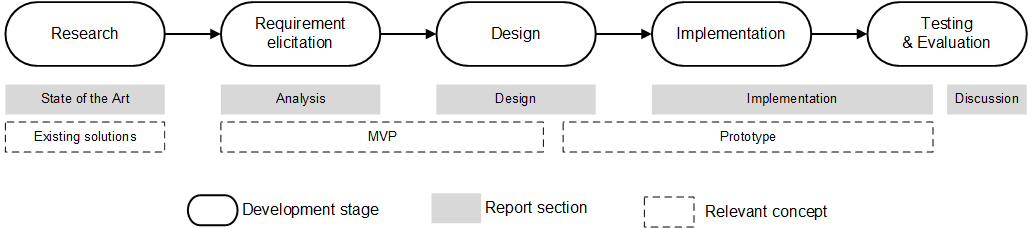
\includegraphics[width=\textwidth]{development-process}
    \caption{The modified waterfall model used in this project (rounded boxes). Below, the corresponding report chapters are shown (grey boxes) and relevant scopes for that stage (dashed boxes).}
    \label{fig:development-process}
\end{figure}

The \textit{initial research} stage is not typically mentioned as a separate stage in literature~\cite{Sommerville2011SoftwareEngineering, CMS2005SELECTINGAPPROACH}, however we list is here separately, as exploring the state-of-the-art technologies and solutions is necessary in a research project. In the requirement elicitation and design, an~\acrfull{mvp} is considered (elaborated on in the following section). From the outputs the design stage, a set of few use-cases is selected, which are then implemented in a prototype
 (the prototype is discussed in section \ref{sec:methodology-prototype}). Integration and maintenance stages are omitted this project, as the goal is not to produce and deploy the software into production.